\documentclass[11pt,a4paper]{article}
\usepackage[T1]{fontenc}
\usepackage{lmodern}
\usepackage[margin=25mm]{geometry}
\usepackage{amsmath,amssymb,amsthm,booktabs,tikz,enumitem,hyperref,microtype}
\definecolor{mulberry}{HTML}{713C58}
\definecolor{spruce}{HTML}{245D57}
\hypersetup{colorlinks=true,linkcolor=spruce,citecolor=spruce,urlcolor=mulberry,
 pdftitle={The maximum Wiener index of trees with prescribed diameter: the sharp second-order constant},
 pdfauthor={Anonymous}}
\newtheorem{theorem}{Theorem}[section]
\newtheorem{lemma}[theorem]{Lemma}
\newtheorem{corollary}[theorem]{Corollary}
\newtheorem{proposition}[theorem]{Proposition}
\theoremstyle{remark}
\newtheorem{remark}[theorem]{Remark}
\newcommand{\eps}{\varepsilon}
\newcommand{\norm}[1]{\lVert #1\rVert}
\setlist{nosep}
\setlength{\emergencystretch}{2em}
\title{The maximum Wiener index of trees with prescribed diameter:\\the sharp second-order constant}
\author{Anonymous\\[3pt]{\small DOI \href{https://doi.org/10.5281/zenodo.24520149}{10.5281/zenodo.24520149}}}
\date{November 2026}
\begin{document}
\maketitle
\begin{abstract}
The Wiener index of a graph is the sum of the distances between all pairs of its vertices. Among trees with $n$ vertices and diameter $d$, the largest Wiener index $M_d(n)$ lies just below $(d/2-\eps/4)n^2$, where $\eps\in\{0,1\}$ is the parity of $d$. Cambie (2020) showed that the shortfall has order $(dn)^{3/2}$ and placed its coefficient between $\sqrt2/3\approx0.4714$ and $29/60\approx0.4833$, in iterated limits. We determine the coefficient: whenever $d\to\infty$ and $d/n\to0$, the shortfall is $(\kappa+o(1))(dn)^{3/2}$ with $\kappa=\sqrt{(175-\sqrt7)/756}\approx0.47747$. The proof rests on a lower bound valid for every way of splitting a branch, which matches, to leading order, a construction that divides each branch into two equal halves at remaining heights decreasing by the factor $1/4$. For each fixed $d\ge4$ we also find the coefficients of $n^{3/2}$ and $n$, with error $O_d(\sqrt n)$; they are computed from the effective resistance of small rooted trees. For large $n$, every maximiser is built from a finite catalogue of branch shapes, so for each fixed $d$ an exact algorithm running in time polynomial in $\log n$ exists. Finally, we give an explicit formula for $M_5(n)$ and all its maximisers for every $n\ge6$.
\end{abstract}

\section{Introduction}
This section explains the problem, what was known, what is new and how the paper is organised.

\subsection{The problem and why it matters}
The \emph{Wiener index} of a connected graph $G$ is $W(G)=\sum_{\{u,v\}}d_G(u,v)$, the sum of the distances between all unordered pairs of vertices. Equivalently, it is $\binom n2$ times the average distance. It was introduced by Wiener in 1947 to predict boiling points of paraffins \cite{wiener}, and it has since become one of the most studied distance invariants in graph theory and chemical graph theory \cite{kst}. A basic extremal question asks how large the average distance can be when the diameter $d$, the largest distance, is prescribed. The question goes back to Plesník \cite{plesnik}. He determined the \emph{least} sum of distances among graphs and digraphs of given order $n$ and diameter $d$ \cite[Thms~2--3]{plesnik}, and observed that ``in the case of upper bounds the problem seems to be much more difficult'' \cite[\S3]{plesnik}. The maximum for given $n$ and $d$ has since been known as Plesník's problem \cite{cambie}; see \cite[Problem~28]{kst}. It remains open in general.

This paper treats the same question for trees. Write
\[
 M_d(n)=\max\{W(T): T \text{ a tree with } n \text{ vertices and diameter } d\}.
\]
A tree of diameter $d$ has every distance at most $d$, so $M_d(n)<d\binom n2$. The exact leading term is $(d/2-\eps/4)n^2$, where $\eps=d\bmod2$, and the interesting quantity is the \emph{deficit}
\[
 \Delta_d(n)=\Big(\frac d2-\frac\eps4\Big)n^2-M_d(n).
\]
For fixed $d$ the deficit grows like $n^{3/2}$, and when $d$ also grows it is of order $(dn)^{3/2}$ \cite{cambie}. We determine its leading constant.

\subsection{What was known}
For $d\le4$ and for $d\ge n-3$ the maximisers are known exactly \cite{wang,wagner}. Mukwembi and Vetrík found sharp upper bounds for $d\le6$; at diameter six their expansion reaches the coefficient of $n$, and at diameter five it reaches $n^{3/2}$ with an $O(n)$ error \cite[Thms~3.3--3.4]{mv}. Cambie gave an asymptotic answer to Plesník's question for graphs and sharper bounds for trees \cite{cambie}. For trees of even diameter $d$ his Theorem~4.8 states
\[
 \frac d2n^2-\Big(\frac{29}{60}d^{3/2}+o(d^{3/2})\Big)n^{3/2}+O_d(n)\ \le\ M_d(n)\ \le\ \frac d2n^2-\Big(\frac{\sqrt2}{3}d^{3/2}+O(\sqrt d)\Big)n^{3/2}+O_d(n),
\]
with the analogous statement for odd $d$; here $n\to\infty$ first and $d\to\infty$ afterwards. His lower construction already used branches that fork into two at geometrically spaced heights, with a numerically optimised ratio of about $0.3825$ \cite[proof of Thm~3.4]{cambie}. He also proved that in every maximiser all leaves are as far from the centre as possible \cite[Lemma~4.1]{cambie}. Recent work determines the maximisers when $d$ is close to $n$ \cite{doublebroom,pandey}.

\subsection{Main results}
Throughout, $d=2r+\eps$ with $\eps\in\{0,1\}$, and $h=r-1$.

\begin{theorem}[The second-order constant]\label{thm:joint}
There are absolute constants $C_1,C_2>0$ and numbers $c_h$ (defined in \eqref{mins} below) such that, for every $h\ge1$ and $n\ge C_1h$,
\[
 \big|\Delta_d(n)-2\sqrt{c_h}\,n^{3/2}\big|\le C_2\,nh^2,\qquad\text{and}\qquad
 \Big|2\sqrt{c_h}-K\big(h+\tfrac12\big)^{3/2}\Big|\le0.49,
\]
where $K=\sqrt8\,\kappa\approx1.35050$. Consequently, for every sequence with $d\to\infty$ and $d/n\to0$,
\[
 \frac{\Delta_d(n)}{(dn)^{3/2}}\longrightarrow\kappa=\sqrt{\frac{175-\sqrt7}{756}}=0.4774744081\ldots .
\]
\end{theorem}

The constant $\kappa$ lies strictly inside Cambie's bracket $[0.4714,0.4833]$. The convergence is genuinely joint: no order of limits is imposed. For fixed $d$ we obtain a three-term expansion. Its constants come from a finite optimisation over small rooted trees, explained in Section~\ref{sec:flow}.

\begin{theorem}[Fixed diameter]\label{main}
For each fixed $d=2r+\eps\ge4$, with $z=1+\eps$,
\[
 M_d(n)=\Big(r+\frac\eps4\Big)n^2-2\sqrt{c_h}\,n^{3/2}-(zr+\beta_h)n+O_d(\sqrt n).
\]
The constants $c_h$ and $\beta_h$ are rational; Table~\ref{tab:constants} lists them for $h\le8$.
\end{theorem}

For example, $M_6(n)=3n^2-2\sqrt6\,n^{3/2}-2n+O(\sqrt n)$, which is the Mukwembi--Vetrík expansion, and
\[
 M_8(n)=4n^2-\sqrt{70}\,n^{3/2}-n+O(\sqrt n).
\]
The maximisers themselves become rigid. Theorem~\ref{rigid} in Section~\ref{sec:exchange} shows that for large $n$ every branch of every maximiser has one of finitely many optimal shapes, with its size and its leaf counts determined up to bounded errors. Two consequences follow. For each fixed $d$ there is an algorithm that computes $M_d(n)$ exactly in time polynomial in $\log n$ (Corollary~\ref{algo}); and for fixed radius $q\ge2$ the maximisers among trees of radius $q$ are, for large $n$, exactly the diameter-$2q$ maximisers. At diameter five no large-$n$ threshold is needed: Theorem~\ref{five} gives $M_5(n)$ and every maximiser for every $n\ge6$.

\subsection{Idea of the proof}
Root the tree at its centre. Cutting an edge separates $b$ vertices from $n-b$, and the edge lies on $b(n-b)$ paths. Summing over edges shows that the deficit is, up to explicit terms, a sum of two costs per branch: a \emph{depth cost} $nA$, which penalises vertices that are not at full depth, and the sum $\sum b_v^2$ of squared subtree sizes along the branch. A branch must carry many leaves at full depth, and those leaves must pass through the branch's internal edges. Think of the leaves as a current flowing from the centre outwards: the squared subtree sizes are then the electrical energy of the current, and the cheapest way to route $b$ leaves through a fixed branch has energy $Rb^2$, where $R$ is an effective resistance. Optimising the number and size of branches turns the two costs into $2\sqrt{AR}\,n^{3/2}$, so everything reduces to minimising $A\cdot R$ over small rooted trees.

For large diameter this minimisation becomes a continuum problem: a mass flows down a tree in the remaining height $\tau$, each edge costs $\int(\tau+m^2)\,d\tau$, and splitting is free. We solve it with an explicit \emph{calibration}, a function $V(\tau,x)$ that is subadditive in the mass and whose growth in $\tau$ is dominated by the running cost. The polynomial $V=\tau^2/2+\tau x^2-x^4/7$ works because its splitting excess is a sum of two squares \eqref{split}. Equality forces equal binary splits at heights $\tau=x^2/2$, so the remaining height at successive splits shrinks by the factor $1/4$ (Figure~\ref{fig:dyadic}).

\subsection{Roadmap}
Section~\ref{sec:flow} sets up the notation and the exact distance identity, and solves the problem for a single branch. Section~\ref{sec:bounds} proves Theorem~\ref{main}. Section~\ref{sec:exchange} proves rigidity, derives the algorithm and reports exact computations showing where rigidity sets in. Section~\ref{sec:mesh} determines the large-height behaviour of $c_h$, and Section~\ref{sec:joint} proves Theorem~\ref{thm:joint}. Section~\ref{sec:constants} computes $c_h$ and $\beta_h$. Section~\ref{sec:five} treats diameters five and four. Section~\ref{sec:scope} discusses limits and open problems. Table~\ref{tab:notation} collects the notation.

\begin{table}[tb]
\centering\small\setlength{\tabcolsep}{4pt}
\begin{tabular}{ll}
\toprule
Symbol & Meaning\\
\midrule
$d=2r+\eps$, $h=r-1$, $z=1+\eps$ & diameter; stem height; number of centres\\
centre & middle vertex ($\eps=0$) or an end of the middle edge ($\eps=1$)\\
depth & distance to the nearer centre; the largest depth is $r$\\
branch & a non-central neighbour of a centre together with all its descendants\\
$b$, $b_v$ & size of a branch; number of descendants of $v$, including $v$\\
stem $H$, $s=|H|$ & a branch without its vertices at depth $r$; its number of vertices\\
tip, outer leaf & stem vertex at depth $h$; vertex at depth $r$\\
proper stem & a stem in which every vertex lies above some tip\\
$A$, $R$, $D$, $\beta$ & depth cost, resistance, voltage sum, tie-breaker \eqref{defs}\\
$c_h$, $\beta_h$ & optimal value of $AR$ and best tie-breaker \eqref{mins}\\
$\tau$, $\Theta=h+\frac12$ & remaining height in Section~\ref{sec:mesh}; its value at the centre\\
$K$, $\kappa$ & $K=f(a)\approx1.35050$ \eqref{K}; $\kappa=K/\sqrt8$\\
\bottomrule
\end{tabular}
\caption{Notation used throughout.}\label{tab:notation}
\end{table}

\section{Stems, flows and the cost of one branch}\label{sec:flow}
This section defines the branch structure of a tree, rewrites the deficit exactly as a sum of branch costs, and computes the cheapest way to load a single branch with leaves.

\paragraph{Centres, branches and stems.} Let $T$ be a tree of diameter $d=2r+\eps$. It has one centre if $\eps=0$ and two adjacent centres if $\eps=1$. The \emph{depth} of a vertex is its distance to the nearer centre, and the greatest depth is $r$. A \emph{branch} begins at a non-central neighbour of a centre and contains all its descendants. Deleting the vertices at depth $r$ from a branch leaves its \emph{stem} $H$; we write $s=|H|$. Vertices at depth $r$ are \emph{outer leaves}, and stem vertices at depth $h=r-1$ are \emph{tips}. A stem is \emph{proper} if it reaches depth $h$ and every stem vertex lies on a path to a tip.

\paragraph{Resistance and voltages.} For a stem $H$ reaching depth $h$, include its entrance edge from the centre, give every edge unit resistance, and wire all tips together; a stem vertex with no tip below it carries no current, so deleting such vertices changes neither $R$ nor the currents elsewhere. Send one unit of current from the centre to the tips, and choose the terminal fractions to minimise $\sum_{v\in H}f_v^2$, where $f_v$ is the current on the edge entering $v$. This strictly convex problem has a unique minimiser, and its value $R$ is the effective resistance. Let $V_v$ be the voltage drop from the centre to $v$, that is, the sum of the currents along the path from the centre to $v$. Define
\begin{align}
 A&=\sum_{v\in H}(r-\operatorname{depth}(v)),&
 D&=\sum_{v\in H}(R-V_v),&
 \beta(H)&=1-2D, \label{defs}\\
 c_h&=\min_H A(H)R(H),&
 \beta_h&=\min_{H:\,A(H)R(H)=c_h}\beta(H). \label{mins}
\end{align}
The minima run over proper stems of height $h$. They are finite computations: the entrance edge gives $R\ge1$ and a single path gives $AR=h^2(h+1)/2$, so only stems with at most $h^2(h+1)/2$ vertices matter.

The circuit can be solved directly. If a vertex has child networks of conductances $C_i$, minimising $\sum_i f_i^2/C_i$ subject to $\sum_if_i=1$ gives fractions $C_i/\sum_jC_j$ and minimum $1/\sum_iC_i$. Adding the entrance edge in series gives $R=1+1/\sum_iC_i$. Induction from a single edge shows that every tip receives positive current and has voltage $V_t=R$; compare the minimum-energy principle \cite[\S1.3.5]{doyle}.

\paragraph{The exact distance identity.} Deleting an edge separates the tree into parts of orders $b$ and $n-b$, and exactly $b(n-b)$ pairs use that edge \cite{wiener}. Orient non-central edges outwards, so that $b_v$ counts the descendants of $v$ including $v$; then $\sum_vb_v$ over non-central vertices is the sum of all depths. For odd $d$ write the two components of the central edge as $n/2\pm\delta$, and set $\delta=0$ for even $d$. The central edge contributes $n^2/4-\delta^2$. A branch with stem $H$ and size $b$ contributes the cost
\begin{equation}
 Q_n=nA+\sum_{v\in H} b_v^2+(b-s), \label{cost}
\end{equation}
where $b-s$ counts the outer leaves, each with $b_v=1$. Summing over edges gives the exact identity
\begin{equation}
 \Big(r+\frac\eps4\Big)n^2-W(T)=zrn+\delta^2+\sum_{\rm branches} Q_n. \label{global}
\end{equation}
Identity \eqref{global} holds for every stem that occurs in a tree, including stems with leaves at depth less than $h$.

\begin{lemma}[Cost of one stem]\label{one}
Fix a stem $H$ reaching depth $h$, and let $F_H(b)$ be the minimum of $Q_n-nA$ over all ways to attach $b-s$ outer leaves to its tips. Then
\begin{equation}
 F_H(b)=R b^2+\beta(H)b+O_H(1)\qquad(b\ge s). \label{exp}
\end{equation}
In every minimising allocation, the number of leaves at tip $t$ differs from $(b-s)f_t$ by $O_H(1)$.
\end{lemma}
\begin{proof}
Index vectors by the edges entering stem vertices, and let $\mathbf b=(b_v)_{v\in H}$. Each vertex of the branch contributes to $\langle f,\mathbf b\rangle$ the sum of $f$ along its path inside the stem; this is $V_v$ for a stem vertex and $R$ for an outer leaf. Hence $\langle f,\mathbf b\rangle=Rb-D$. Since $f$ is the optimal unit current, $\langle f,f\rangle=R$, and expanding $\norm{\mathbf b-bf}^2$ gives the exact identity
\begin{equation}
 Q_n=nA+Rb^2+(1-2D)b-s+\norm{\mathbf b-bf}^2. \label{exact}
\end{equation}
Round the numbers $(b-s)f_t$ to integers with the same sum, each error below one. Then every $b_v$ differs from $bf_v$ by at most $s$ plus the number of tips, so the minimal squared norm is bounded independently of $b$. Its tip coordinates give the last assertion, since $b_t$ includes the tip itself.
\end{proof}

\section{Fixed diameter: matching bounds and exclusion of other shapes}\label{sec:bounds}
This section proves Theorem~\ref{main}. A good construction keeps the total excess over the ideal cost at order $\sqrt n$, whereas any branch whose stem is not optimal costs order $n$ extra; so large maximisers use only optimal stems, and summing the exact costs gives the expansion.

Fix $d\ge4$ and abbreviate $c=c_h$, $\beta=\beta_h$ and $L_n=2\sqrt{cn}+\beta$. The \emph{excess} of a branch is $G=Q_n-L_nb$.

\paragraph{Construction.} Choose a proper stem attaining both minima in \eqref{mins} and put $b_0=\sqrt{cn}/R=\sqrt{nA/R}$. At a single centre use the integer nearest to $(n-1)/b_0$ branches. With two centres, split the $n-2$ non-central vertices evenly to within one and apply the same rule on each side. Make the branch sizes on a side as equal as possible. There are $\Theta_d(\sqrt n)$ branches, each of size $b_0+O_d(1)$, because rounding the number of branches moves the mean size by $O_d(1)$. Load each branch as in Lemma~\ref{one}. For large $n$ every tip carries leaves and there are at least two full-height branches, so the diameter is exactly $d$. Since $AR=c$, the identity $nA+Rb^2-2\sqrt{cn}\,b=R(b-b_0)^2$ shows that every branch has $G=O_d(1)$, and therefore
\begin{equation}
 \delta^2+\sum G=O_d(\sqrt n). \label{trial}
\end{equation}
Since $\sum b=n-z$ for every tree, \eqref{global} shows that every maximiser also satisfies \eqref{trial}. In particular its deficit is $O_d(n^{3/2})$. Each branch costs at least $n$ in \eqref{cost}, so a maximiser has $O_d(\sqrt n)$ branches.

\begin{lemma}[A uniform gap]\label{gap}
There are $n_0(d)$ and $\eta_d>0$ such that for $n\ge n_0(d)$ every branch whose stem is not a proper stem with $AR=c$ has $G\ge\eta_dn$. For a proper stem with $AR=c$,
\[
 G\ge R(b-b_0)^2+(\beta(H)-\beta)b-s,\qquad b_0=\sqrt{cn}/R .
\]
\end{lemma}
\begin{proof}
We treat three cases. (i) If $A>c+1$: the entrance edge alone gives $G\ge nA+b^2-L_nb\ge nA-L_n^2/4$, a gap of at least $n/2$ for large $n$. (ii) The remaining stems have $A\le c+1$; each stem vertex adds at least one to $A$, so they form a finite set. A stem not reaching depth $h$ has no outer leaves, so $b=s=O_d(1)$ and $A\ge1$ gives a linear gap. (iii) A stem reaching depth $h$: deleting every stem vertex that has no tip below it preserves $R$ and strictly decreases $A$ whenever something is pruned, so $AR\ge c$, with equality only for a proper stem. If $AR>c$, completing the square in \eqref{exact} gives
\[
 G\ge nA-\frac{(2\sqrt{cn}+\beta-\beta(H))^2}{4R}-s=n(A-c/R)+O_d(\sqrt n).
\]
Take $\eta_d$ below the smallest of these finitely many positive gaps. For $AR=c$ the displayed bound follows directly from \eqref{exact}.
\end{proof}

\begin{proof}[Proof of Theorem~\ref{main}]
Consider a maximiser with $n\ge n_0(d)$. Every branch with an optimal stem has $G\ge-s=-O_d(1)$ by Lemma~\ref{gap}, since $\beta(H)\ge\beta$; there are $O_d(\sqrt n)$ branches, so these branches contribute at least $-O_d(\sqrt n)$ to $\sum G$. If some branch had a non-optimal stem, \eqref{trial} would give $\eta_dn-O_d(\sqrt n)\le\delta^2+\sum G\le O_d(\sqrt n)$, which fails for large $n$. Hence every branch has $AR=c$, and adding the inequalities of Lemma~\ref{gap} gives
\begin{equation}
 \delta^2+\sum\big[R(b-b_0)^2+(\beta(H)-\beta)b\big]=O_d(\sqrt n).
 \label{squares}
\end{equation}
In particular $|\delta^2+\sum G|=O_d(\sqrt n)$. Substituting into \eqref{global} gives deficit $zrn+L_n(n-z)+O_d(\sqrt n)$, which is Theorem~\ref{main}.
\end{proof}

Equation \eqref{squares} also shows that every branch has $b=b_0+O_d(n^{1/4})$, so $b=\Theta_d(\sqrt n)$, and that a stem with $\beta(H)>\beta$ occurs on only $O_d(1)$ branches.

\section{Rigidity, exact computation and where rigidity begins}\label{sec:exchange}
This section moves single leaves between branches to pin down every branch size to within a constant, deduces an exact algorithm for fixed $d$, and reports exact computations, for $6\le d\le11$ and $n\le3000$, of the orders at which maximisers use only optimal stems.

\begin{theorem}[Rigidity]\label{rigid}
Fix $d\ge4$. For all sufficiently large $n$, every branch of every maximiser has a proper stem $H$ with $AR=c_h$, at most $O_d(1)$ branches have $\beta(H)>\beta_h$, and a branch of size $b$ satisfies
\[
 b=\frac{\sqrt{c_h n}}{R(H)}+O_d(1).
\]
At each tip $t$ the number of attached leaves is $(b-|H|)f_t+O_d(1)$. For odd $d$, each component obtained by removing the central edge has $n/2+O_d(1)$ vertices.
\end{theorem}
\begin{proof}
On each side of a maximiser the total size is $\Theta(n)$ by \eqref{squares}, and there are $\Theta_d(\sqrt n)$ branches, so \eqref{squares} supplies an \emph{anchor} branch with $|b-b_0|=O_d(1)$. Each branch minimises its own cost for its stem and size: otherwise replacing its allocation by the one of Lemma~\ref{one} would increase $W$, and the new branch still reaches full depth. On the finite set of optimal stems, \eqref{exp} gives
\begin{equation}
 F_H(b+1)-F_H(b)=2Rb+O_d(1),\qquad
 F_H(b)-F_H(b-1)=2Rb+O_d(1). \label{diff}
\end{equation}
Move one outer leaf from one branch to another on the same side and re-optimise both allocations. Both directions are legal, because by Lemma~\ref{one} every tip carries $\Theta_d(\sqrt n)$ leaves, so the donor keeps full depth. Optimality and \eqref{diff} give $|R_ib_i-R_jb_j|=O_d(1)$ for any two branches. The anchor has $R_jb_j=\sqrt{cn}+O_d(1)$, which proves the size bound; the tip bound follows from Lemma~\ref{one}. For odd $d$, moving one leaf from the larger side to the smaller changes the two branch costs by $O_d(1)$ and changes $\delta^2$ by $1-2|\delta|$; optimality forces $|\delta|=O_d(1)$.
\end{proof}

\begin{corollary}[Exact computation]\label{algo}
For each fixed $d$ there is an algorithm that computes $M_d(n)$, together with a maximiser encoded by branch multiplicities, in time polynomial in $\log(n+1)$. Its preprocessing and constants depend on $d$.
\end{corollary}
\begin{proof}
For $d=2,3$ the star and the balanced double star are optimal; for $d=1$ only $n=2$ is admissible. For $d\ge4$, enumerate the finitely many stems in \eqref{mins} and retain every stem with $AR=c_h$, including ties in the second minimum. List the branch sizes in the bounded windows of Theorem~\ref{rigid} and all integer tip loads in their bounded windows, with the correct sum. This gives $O_d(1)$ \emph{decorated types}, each a fully specified branch whose size and cost \eqref{cost} are integers of bit length $O_d(\log(n+1))$; exact floors of rational multiples of square roots are computed by integer square roots. Introduce one non-negative integer multiplicity per type and per side, impose each side's vertex total as a linear equality, and require two full-depth branches at a single centre or at least one on each side of a central edge. For odd $d$, enumerate the boundedly many side totals near $n/2$, so the central term is constant within each programme. Minimise the total branch cost. Every feasible vector gives a tree, and by Theorem~\ref{rigid} every maximiser appears among the optimal vectors. Each programme has a fixed number of variables, a linear objective and linear constraints, so Lenstra's algorithm \cite{lenstra}, with binary search on the integer objective, solves it in time polynomial in the bit length. The algorithm returns one optimal vector; listing every maximiser may take longer.

All bounds used for fixed $d$ are effective. The trial norm in \eqref{exact} is at most $s(2s+\#\text{tips})^2$; the gap test discards $A>c+1$ at once and otherwise uses the least positive value of $A-c/R$; the constants in \eqref{squares} use the largest $s$ and the least positive $\beta(H)-\beta$; and the errors in \eqref{diff} are bounded by the range of the norm term plus $R+|\beta(H)|$. With rational outward rounding these give the windows and a threshold through elementary inequalities in $n^{1/4}$. Below that threshold one enumerates directly.
\end{proof}

Corollary~\ref{algo} is an existence statement; we have not implemented the integer-programming step. In practice, for small $d$, an exact dynamic programme over branches is simpler, and we use one next.

\paragraph{Where rigidity begins.} The proof of Theorem~\ref{rigid} gives effective thresholds, but we have not evaluated them. To see the finite-$n$ behaviour we computed $M_d(n)$ exactly for $6\le d\le11$ and all orders $2r+4\le n\le3000$ with a dynamic programme over branches. By Cambie's lemma \cite[Lemma~4.1]{cambie} every leaf of a maximiser lies at depth $r$, so a maximiser consists of full-height branches, and identity \eqref{global} lets each branch be optimised separately for each size. The programme records whether the best tree can be built from optimal stems only, and whether some maximiser uses a non-optimal stem. For $d=6$ and $d=7$, at every order tested ($n\ge10$), every maximiser is built from optimal stems only. For $d=8,9,10,11$ the last orders at which some maximiser still uses a non-optimal stem are $597$, $1034$, $288$ and $289$ respectively; above them, up to $n=3000$, every maximiser uses optimal stems only. Below these orders the picture is irregular. For example, at $d=8$ there are $348$ orders $n\le596$ at which no maximiser is built from optimal stems only, and $n=249$, discussed in Section~\ref{sec:constants}, is one of them. These computations are consistent with the first assertion of Theorem~\ref{rigid} and show where it starts to hold in the tested range; they do not test its size and leaf-count windows.

\paragraph{Fixed radius.} Stevanović, Milosavljević and Vukičević studied by computer the maximisers among trees of given radius \cite[\S5]{radius}. They found that a simple family of trees (broom-fans) is extremal for small orders, but not for $24$ vertices and radius $7$, and suggested that a simple general description may be out of reach. For fixed radius $q\ge2$ and large order the question has a clean answer. A tree of radius $q$ has diameter $2q-1$ or $2q$, and the leading coefficients of $M_{2q-1}$ and $M_{2q}$ are $q-3/4$ and $q$. Hence, for all sufficiently large $n$, the maximisers among trees of radius $q$ are exactly the diameter-$2q$ maximisers, and Theorem~\ref{rigid} and Corollary~\ref{algo} apply to them.

\section{The large-diameter constant}\label{sec:mesh}
This section shows that $2\sqrt{c_h}$ equals $K(h+\frac12)^{3/2}$ up to a bounded error. The lower bound comes from a calibration valid for every way of splitting the current; the upper bound comes from an explicit construction with equal binary splits.

Define
\begin{equation}
 a=\sqrt{\frac{7-\sqrt7}6},\qquad a_+=\sqrt{\frac{7+\sqrt7}6},\qquad
 f(\sigma)=\frac1{2\sigma}+\sigma-\frac{\sigma^3}7,\qquad K=f(a).
 \label{K}
\end{equation}
Since $f'(\sigma)=-(6\sigma^4-14\sigma^2+7)/(14\sigma^2)$, $f$ decreases on $(0,a]$, increases on $[a,a_+]$ and decreases on $[a_+,\infty)$. Numerically $a\approx0.85189$, $a_+\approx1.26792$ and $K\approx1.35050$, and $K/\sqrt8=\kappa$.

\begin{theorem}\label{mesh}
Write $\Theta=h+1/2$. For every $h\ge1$,
\[
 K\Theta^{3/2}-\sqrt{\frac{175+\sqrt7}{756}}
 \ \le\ 2\sqrt{c_h}\ \le\
 K\Theta^{3/2}-\frac{3}{7\sqrt2}.
\]
\end{theorem}
The two constants are $0.48475$ and $0.30305$. The lower bound is nearly attained at $h=1$, where $2\sqrt{c_1}-K\Theta^{3/2}=-0.48103$.

\paragraph{The continuum reformulation.} Give a stem a root mass $x>0$ and let $m_e$ be a conserved non-negative flow from the root to the tips. The least value of $\sum_em_e^2$ is $Rx^2$, so
\[
 2\sqrt{c_h}=\min\Big\{\frac{A+\sum_em_e^2}{x}\Big\},
\]
the minimum running over proper stems, flows and $x>0$; indeed $(A+Rx^2)/x\ge2\sqrt{AR}$ with equality at $x=\sqrt{A/R}$. Represent an edge whose lower end has depth cost $j$ by the interval $[j-\frac12,j+\frac12]$ of \emph{remaining height} $\tau$. Its contribution to $A+\sum m_e^2$ is then exactly $\int(\tau+m_e^2)\,d\tau$ over that interval. A stem becomes a tree drawn downwards from $\tau=\Theta$ at the centre to $\tau=\frac12$ at the tips, carrying mass that may split at vertices.

\begin{lemma}[A lower bound valid at every split]\label{cal}
There is a continuous function $V(\tau,x)$ for $\tau,x\ge0$, with $V(0,x)=0$ for $x>0$, such that
\[
 V(\tau,x)\ge Kx\tau^{3/2},\qquad V(\tau,y+z)\le V(\tau,y)+V(\tau,z),
 \qquad V(\tau_2,x)-V(\tau_1,x)\le\int_{\tau_1}^{\tau_2}(\tau+x^2)\,d\tau
\]
for all $y,z\ge0$, $x>0$ and $0\le\tau_1<\tau_2$.
\end{lemma}
\begin{proof}
Integrating the edge cost suggests $\tau^2/2+\tau x^2$ plus a function of the mass. For two equal children of mass $x/2$, the excess of $\tau^2/2+\tau x^2-\alpha x^4$ at a split is minimal at $\tau=x^2/2$, and that minimum is zero exactly when $\alpha=1/7$. So put $g(\tau,x)=\tau^2/2+\tau x^2-x^4/7$. Its excess at a binary split factors as
\begin{equation}
 g(\tau,y)+g(\tau,z)-g(\tau,y+z)
   =\tfrac12(\tau-2yz)^2+\tfrac47 yz(y-z)^2. \label{split}
\end{equation}
An equal split of mass $x$ is therefore free exactly at $\tau=x^2/2$.

The negative quartic term needs a modification at large mass. Since $f(1)=19/14>K$ and $f(\sqrt2)=27\sqrt2/28>K$, and $\sqrt2>a_+$, the last root $\sigma_*$ of $f(\sigma)=K$ exceeds $\sqrt2$ (numerically $\sigma_*\approx1.50366$), and $f\ge K$ on $(0,\sigma_*]$. Define $V=g$ when $x\le\sigma_*\sqrt\tau$ and $V=Kx\tau^{3/2}$ otherwise. Because $g(\tau,x)=x\tau^{3/2}f(x/\sqrt\tau)$, the two pieces agree on the boundary, $V$ is continuous, and $V\ge Kx\tau^{3/2}$ everywhere. Also $V(0,x)=0$ for $x>0$, and $V(\tau,0)=\tau^2/2\ge0$.

\emph{Subadditivity.} A child never carries more mass than its parent. If the parent lies in the polynomial piece, so do both children, and \eqref{split} applies. If the parent lies in the linear piece, $V(\tau,y+z)=K(y+z)\tau^{3/2}\le V(\tau,y)+V(\tau,z)$ by the lower bound. Iterating covers any finite number of children.

\emph{Growth in $\tau$.} On the polynomial piece $\partial_\tau g=\tau+x^2$ exactly. On the linear piece $\partial_\tau V=\frac32Kx\sqrt\tau$, and $\frac32Kx\sqrt\tau\le\tau+x^2$ is equivalent to $\sigma+1/\sigma\ge3K/2$ with $\sigma=x/\sqrt\tau\ge\sigma_*$; this holds because $\sigma+1/\sigma$ increases for $\sigma\ge1$ and $\sqrt2+1/\sqrt2>3K/2$. For fixed $x$, the map $\tau\mapsto V(\tau,x)$ is continuous and continuously differentiable except at the single point $\tau=x^2/\sigma_*^2$ where the pieces meet. It is therefore absolutely continuous, and integrating $\partial_\tau V\le\tau+x^2$ gives the third property, also along an edge that crosses the boundary between the pieces.
\end{proof}

\begin{figure}[tb]
\centering
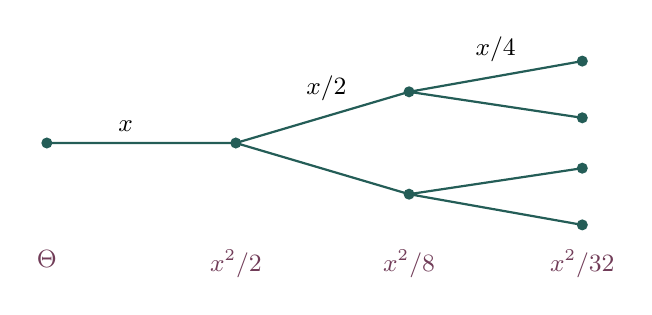
\begin{tikzpicture}[x=1cm,y=1cm,thick,font=\small]
\draw[spruce] (0,0)--(2.4,0) (2.4,0)--(4.6,.65) (2.4,0)--(4.6,-.65)
(4.6,.65)--(6.8,1.04) (4.6,.65)--(6.8,.32)
(4.6,-.65)--(6.8,-.32) (4.6,-.65)--(6.8,-1.04);
\foreach \x/\y in {0/0,2.4/0,4.6/.65,4.6/-.65,6.8/1.04,6.8/.32,6.8/-.32,6.8/-1.04}
  \fill[spruce] (\x,\y) circle (2pt);
\node[above] at (1.0,.02) {$x$};
\node[above] at (3.55,.41) {$x/2$};
\node[above] at (5.7,.90) {$x/4$};
\node[below,text=mulberry] at (0,-1.23) {$\Theta$};
\node[below,text=mulberry] at (2.4,-1.23) {$x^2/2$};
\node[below,text=mulberry] at (4.6,-1.23) {$x^2/8$};
\node[below,text=mulberry] at (6.8,-1.23) {$x^2/32$};
\end{tikzpicture}
\caption{Two successive equal splits in the optimal pattern. Edge labels are masses; the labels below give the remaining height $\tau$ at the root, at the two visible splits, and at the next prospective split. Each split occurs where its excess in \eqref{split} vanishes, so the remaining height falls by the factor $1/4$ from one split to the next. Horizontal spacing is schematic.}\label{fig:dyadic}
\end{figure}

\begin{proof}[Proof of Theorem~\ref{mesh}, lower bound]
Choose a stem attaining $c_h$, its optimal current, and $x=\sqrt{A/R}$, so that $(A+\sum m_e^2)/x=2\sqrt{c_h}$. Apply the third property of Lemma~\ref{cal} on every edge and subadditivity at every vertex. Every stem leaf is a tip at remaining height $\frac12$; writing $y_i$ for the loads at the tips,
\[
 A+\sum_e m_e^2\ge V(\Theta,x)-\sum_i V(\tfrac12,y_i).
\]

\emph{Every tip load satisfies $y\ge1/\sqrt2$.} Take a tip with load $y$, and let its nearest branching ancestor be $\ell$ edges above it (if there is no branching vertex, the stem is a path and $y=x=\sqrt{(h+1)/2}\ge1$). Delete the $\ell$ stem vertices on the unbranched path from that ancestor down to the tip, and send its load down a path of the same length $\ell$ to a tip below a different child of the same ancestor. The new stem still reaches depth $h$. Its depth cost falls by $\ell(\ell+1)/2$. The deleted path loses energy $\ell y^2$; the receiving path gains $2yP+\ell y^2$, where $P=\ell y$ is the common voltage drop along both paths (all tips have the same potential). The net energy change is $2\ell y^2$. Since $(A'+\sum m'^2_e)/x\ge2\sqrt{A'R'}\ge2\sqrt{c_h}$ for every stem and flow with root mass $x$, minimality gives $2\ell y^2\ge\ell(\ell+1)/2$, so $y^2\ge(\ell+1)/4\ge\frac12$.

\emph{Terminal estimate.} Put $\sigma=y\sqrt2\ge1$. On the polynomial piece $V(\frac12,y)/y=f(\sigma)/\sqrt8$, and on the linear piece it equals $K/\sqrt8$. Over $\sigma\ge1$ the maximum is $f(a_+)/\sqrt8=\sqrt{(175+\sqrt7)/756}$, attained at $\sigma=a_+<\sigma_*$. Since $\sum_iy_i=x$ and $V(\Theta,x)\ge Kx\Theta^{3/2}$, dividing by $x$ proves the lower bound.
\end{proof}

\begin{proof}[Proof of Theorem~\ref{mesh}, upper bound]
Start with root mass $x=a\sqrt\Theta$ and split all masses equally, level by level. A parent of mass $x/2^k$ splits without excess at $\tau_k=x^2/(2\cdot4^k)$. Let $J$ be least with $\tau_J<1$. If $J=0$, the construction is a path; this happens only for $\Theta<2/a^2\approx2.76$, that is $h\le2$, and then $y=x=a\sqrt\Theta\in[1/\sqrt2,\sqrt2]$. Otherwise, for $k<J$, place the $k$-th split at the half-integer level nearest to $\tau_k$. Because $a^2$ is irrational, every $\tau_k$ is irrational, so the nearest half-integer is unique and each rounding error is less than $\frac12$. For $k+1<J$ we have $\tau_k-\tau_{k+1}=3\tau_{k+1}\ge3$, so the rounded levels differ by more than $2$, hence by at least $3$; distinct splits therefore lie at distinct vertices. The first rounded level is at most $0.363\Theta+\frac12\le\Theta-1$ (as $\Theta\ge2/a^2>2.36$), so the first split lies inside the branch, and the last is at least $\frac32$ because $\tau_{J-1}\ge1$. The $2^J$ tips all carry $y=x/2^J$, and $y^2=2\tau_J<2$, $y^2=\tau_{J-1}/2\ge\frac12$, so $y\in[1/\sqrt2,\sqrt2]$.

Telescope $g$ along the edges from $\Theta$ down to the tips at $\frac12$. The cost of each edge equals the change in $g$ along it, a split displaced by $|\delta|<\frac12$ from its ideal height has excess $\delta^2/2\le\frac18$ by \eqref{split}, and there are $2^J-1$ splits. Hence the cost per unit root mass is at most
\[
 \frac{g(\Theta,x)+(2^J-1)/8-2^Jg(\frac12,y)}{x}\le K\Theta^{3/2}+\frac{1/8-g(\frac12,y)}{y}
   =K\Theta^{3/2}-\frac y2+\frac{y^3}7,
\]
using $g(\Theta,x)=xK\Theta^{3/2}$ at $x=a\sqrt\Theta$. The cubic $-y/2+y^3/7$ is convex and equals $-3/(7\sqrt2)$ at both ends of $[1/\sqrt2,\sqrt2]$, which proves the upper bound.
\end{proof}

\begin{remark}\label{rem:cambie-ratio}
Cambie's construction also forks into two at geometrically spaced heights \cite[proof of Thm~3.4]{cambie}, with ratio about $0.3825$. Identity \eqref{split} explains the optimal choice: equal halves, at remaining heights in ratio $1/4$, so that the mass at a split is $\sqrt{2\tau}$. Lemma~\ref{cal} then shows that no other stem does better at leading order, whatever its degrees or the sizes of its splits. The function $V$ plays the role of a value function in a verification argument for a one-dimensional branched-transport problem with running cost $\tau+m^2$.
\end{remark}

\section{Simultaneous growth of order and diameter}\label{sec:joint}
This section proves Theorem~\ref{thm:joint}. The fixed-diameter error terms of Section~\ref{sec:bounds} may grow with $d$, so here we prove a bound whose constants are absolute; Theorem~\ref{mesh} then evaluates the main term.

\begin{lemma}[Optimal stems are small]\label{opt-size}
For a stem minimising $AR$ at height $h$, the optimal root mass $x=\sqrt{A/R}$ satisfies $\sqrt{(h+1)/2}\le x\le\frac32K\sqrt\Theta+0.19$, the stem has $O(h)$ vertices and it has $O(\sqrt h)$ tips. The implied constants are absolute.
\end{lemma}
\begin{proof}
In the lower-bound proof of Theorem~\ref{mesh}, the nonnegative excesses along edges and at splits sum to $2\sqrt{c_h}\,x-V(\Theta,x)+\sum_iV(\frac12,y_i)$. By both halves of Theorem~\ref{mesh} this is at most $C_0x$, with $C_0=\sqrt{(175+\sqrt7)/756}-3/(7\sqrt2)<0.19$. If $x>\sigma_*\sqrt\Theta$, the first edge lies in the linear piece and alone has excess $\int_{\Theta-1}^{\Theta}(\tau+x^2-\frac32Kx\sqrt\tau)\,d\tau\ge x^2-\frac32Kx\sqrt\Theta$, so $x\le\frac32K\sqrt\Theta+C_0$; if $x\le\sigma_*\sqrt\Theta$ the same bound holds since $\sigma_*<\frac32K$. For the lower bound on $x$: sending all current down one path shows $R\le h$, and some path of $h$ stem vertices gives $A\ge h(h+1)/2$.

Now fix a vertex with at least two children, choose one child subtree in which every path to a tip has $j$ edges (counting its entrance edge), delete it, and send its mass $y$ to a single tip of a sibling subtree along a path of $j$ edges. The depth cost falls by at least $j(j+1)/2$. Let $\delta$ be the change in edge flow: $-m_e$ on the deleted edges and $+y$ on the $j$ receiving edges. The energy changes by $2\langle m,\delta\rangle+\norm\delta^2$. The first term vanishes: the deleted subtree's energy equals $yP$, where $P$ is the common voltage drop from the fork to the tips, and the receiving path also carries drop $P$. On each of the $j$ deleted levels the masses are nonnegative with sum $y$, so their squares sum to at most $y^2$; hence $\norm\delta^2\le2jy^2$. Optimality gives $2jy^2\ge j(j+1)/2$, so $y\ge\sqrt{j+1}/2$. Above the first fork the mass is $x\ge\sqrt{(h+1)/2}\ge\sqrt{j+1}/2$, and unary continuations preserve mass; so every edge with $j$ levels remaining carries at least $\sqrt{j+1}/2$. The masses at each level sum to $x$, so there are at most $2x/\sqrt{j+1}$ such edges, and summing over $j\le h$ gives at most $4x\sqrt h=O(h)$ stem vertices. The case $j=1$ bounds the number of tips by $2x=O(\sqrt h)$.
\end{proof}

\begin{proof}[Proof of Theorem~\ref{thm:joint}]
The bound on $2\sqrt{c_h}$ is Theorem~\ref{mesh}, since $0.30<0.49$ and $0.485<0.49$.

\emph{Lower bound on the deficit.} Take a maximiser. Cambie's peripheral-leaf lemma \cite[Lemma~4.1]{cambie} states that no leaf of a maximiser is at distance less than $(d-1)/2$ from a central vertex; it holds for every maximiser and every $n$. Applied to the nearer centre, it puts every leaf at depth exactly $r$ for both parities. So every stem vertex has a tip below it. Assign the unit mass of each stem vertex to one such tip, and each outer leaf to its parent tip. The resulting conserved edge flows $F_v$ have total $b$ in each branch, and $b_v\le F_v\le b_v+h$, since only units from the at most $h-1$ strict stem ancestors of $v$ can be added to its count. There are at most $n$ stem edges and $\sum b_v\le hn$, because each vertex is counted by at most $h$ stem edges. Hence
\[
 \sum F_v^2-\sum b_v^2\le 2h\sum b_v+h^2 n\le3h^2n.
\]
For each branch, $nA+\sum F_v^2\ge nA+Rb^2\ge2\sqrt{c_h n}\,b$. The remaining terms of \eqref{global} are nonnegative. Summing over branches and using $\sum b=n-z$, then replacing $n-z$ by $n$ at cost $O(h^{3/2}\sqrt n)$, gives $\Delta_d(n)\ge2\sqrt{c_h}n^{3/2}-O(nh^2)$.

\emph{Upper bound on the deficit.} Use a stem attaining $c_h$, with $x=\sqrt{A/R}$, $s=O(h)$ vertices and $O(\sqrt h)$ tips (Lemma~\ref{opt-size}). Give the two sides nearly equal vertex totals for odd $d$. On a side with $u$ non-central vertices take the nearest integer $k$ to $u/(x\sqrt n)$ copies of the stem and balance the branch sizes. Since $|u/k-x\sqrt n|\le x\sqrt n/(2k)$, Lemma~\ref{opt-size} gives $k\asymp\sqrt{n/h}$, $b=x\sqrt n+O(h)$ and $b\asymp\sqrt{nh}$, where $\asymp$ means bounded above and below by absolute constant multiples. Attach $b-s$ outer leaves according to the optimal tip shares, rounding each within one and keeping the sum. By the tip-load bound $y\ge1/\sqrt2$ in the proof of Theorem~\ref{mesh}, each share is at least $1/(\sqrt2x)$. The threshold $n\ge C_1h$ is used in three places: to make $k\ge2$ (or $k\ge1$ on each side), to make $(b-s)/(\sqrt2x)\ge1$ so that every tip receives a leaf and the diameter is exactly $d$, and to make $h^{5/2}\sqrt n\le h^2n$ below.

The actual loads satisfy $|b_v-bf_v|\le s+\#\text{tips}=O(h)$ on each stem edge, and on each of the $h$ levels the currents $f_v$ sum to one. Hence
\[
 \sum_{v\in H} b_v^2 = Rb^2 + O(bh^2+h^3)=Rb^2+O(bh^2).
\]
Further, $nA+Rb^2=2\sqrt{c_hn}\,b+R(b-x\sqrt n)^2$. Summed over $O(\sqrt{n/h})$ branches, the squared remainder is $O(h^{5/2}\sqrt n)=O(h^2n)$, using $R\le h$. The central terms, the outer leaves and the bounded imbalance contribute $O(hn)$ to \eqref{global}. This proves the uniform estimate.

\emph{The limit.} Put $\Theta=h+\frac12=(d-1-\eps)/2$. By the two estimates, $\Delta_d(n)=K\Theta^{3/2}n^{3/2}+O(n^{3/2})+O(nh^2)$. Dividing by $(dn)^{3/2}$ and using $\Theta/d\to\frac12$ and $nh^2/(dn)^{3/2}=O(\sqrt{d/n})$ gives the limit $K/2^{3/2}=\kappa$.
\end{proof}

\begin{remark}[What the limit needs]\label{rem:limit-only}
The limit alone needs less than the uniform estimate. The lower bound above uses only Cambie's lemma and $AR\ge c_h$, and is valid for all $n$. For the upper bound any explicit stem with $2\sqrt{AR}\le K\Theta^{3/2}+O(1)$, $O(h)$ vertices, $O(\sqrt h)$ tips and tip shares at least of order $1/\sqrt h$ suffices; the construction in the proof of Theorem~\ref{mesh} has these properties (equal shares $2^{-J}$, $2^J=O(\sqrt h)$ tips, and $O(\Theta)$ vertices because the gaps between splits decrease geometrically). Lemma~\ref{opt-size} is needed only for the rate $O(nh^2)$.
\end{remark}

\begin{remark}[Rate and mean distance]\label{rem:rate}
The relative error in the limit is $O(1/d+\sqrt{d/n})$, and the first term converges slowly because $\Theta=(d-1-\eps)/2$ differs from $d/2$ by a constant. For example, at $d=18$ the exact coefficient gives $2\sqrt{c_8}/18^{3/2}\approx0.433$, about $9\%$ below $\kappa$, whereas $K(h+\frac12)^{3/2}\approx33.47$ is close to $2\sqrt{c_8}\approx33.05$; so $K(h+\frac12)^{3/2}n^{3/2}$ is a much better approximation to the deficit than $\kappa(dn)^{3/2}$. Similarly, at $d=9$ and $n=3000$ the normalised deficit $\Delta_9(3000)/(27000)^{3/2}$ is only about $0.313$, while the three-term expansion of Theorem~\ref{main} is accurate there, with an error of about $10.7\sqrt n$. In terms of the largest mean distance $\bar d_{\max}=2M_d(n)/(n(n-1))$, which is the normalisation of Plesník's question, Theorem~\ref{thm:joint} reads
\[
 d-\bar d_{\max}=\frac\eps2+(2\kappa+o(1))\,\frac{d^{3/2}}{\sqrt n}\qquad(d\to\infty,\ d/n\to0).
\]
At the other extreme, $d=n-1$ forces a path, with Wiener index $(n^3-n)/6$, and the normalised deficit then tends to $1/3$.
\end{remark}

\section{Evaluating the constants}\label{sec:constants}
This section computes $c_h$ and $\beta_h$ exactly by a recursion over small rooted trees and checks the results against known cases.

The recursion for splitting currents gives an exact rational computation without listing labelled trees. At each height and each integer depth cost $A$, retain the greatest conductance $C=1/R$, and among stems with that conductance the greatest $D$ of \eqref{defs}. If the child stems have pairs $(C_i,D_i)$ and $S=\sum_iC_i$, the new pair is
\[
 C=\frac{S}{1+S},\qquad D=\frac{1+\sum_i C_iD_i}{S}.
\]
Indeed the new root is one voltage drop $1/S$ away from the tips, and inside child $i$ all drops are scaled by $C_i/S$. Adding a root costs its height plus the sum of the child costs. An unbounded integer knapsack over child costs maximises $(\sum C_i,\sum C_iD_i)$ in lexicographic order. This loses no optimum: every child of a stem attaining $c_h$ must have the greatest conductance for its cost, since otherwise $R$ would fall at the same $A$, and $D$ increases with each $D_i$. A single edge starts at $(A,C,D)=(1,1,0)$, and the bound after \eqref{mins} truncates the computation. To list all stems attaining $c_h$, as Corollary~\ref{algo} requires, one retains all ties instead.

\begin{table}[tb]
\centering
\begin{tabular}{crrrrrrrr}
\toprule
$h$ & 1&2&3&4&5&6&7&8\\
\midrule
$d$ & 4, 5&6, 7&8, 9&10, 11&12, 13&14, 15&16, 17&18, 19\\
$c_h$ & 1&6&$35/2$&$77/2$&72&120&186&273\\
$\beta_h$ & 1&$-1$&$-3$&$-8$&$-15$&$-21$&$-31$&$-43$\\
\bottomrule
\end{tabular}
\caption{The constants of Theorem~\ref{main} for $h=r-1\le8$.}\label{tab:constants}
\end{table}

For $h=2$ a root with $k$ tips has $AR=(2+k)(1+1/k)$. Both $k=1$ and $k=2$ attain $6$, with $\beta$ values $-1$ and $0$. Theorem~\ref{main} therefore gives $M_6(n)=3n^2-2\sqrt6\,n^{3/2}-2n+O(\sqrt n)$, in agreement with Mukwembi and Vetrík \cite[Thm~3.4]{mv}. For $h=3$ the unique optimal stem runs two edges from the centre and then forks into two tips. It has $A=3+2+1+1=7$ and $R=1+1+\frac12=\frac52$, which gives $2\sqrt{c_3}=\sqrt{70}$ and the expansion of $M_8$ in the introduction. Ties are not rare: at $h=5$ the stems with $(A,R)=(16,\frac92)$ and $(18,4)$ both attain $72$, and at $h=8$ the stems with $(39,7)$ and $(42,\frac{13}2)$ both attain $273$.

At $n=249$ the exact maximum is $M_8(249)=215016$. One maximiser has three branches whose stems are paths, each carrying $19$ outer leaves, and seven branches with the optimal forked stem, each carrying $11$ outer leaves per tip. The path stem has $AR=18>c_3$, so this order is still below the rigidity threshold. Cambie's thesis shows a tree with the same two stem shapes \cite[Samenvatting, Fig.~12.17]{thesis}; the leaf counts printed there ($19$ and $10$) give a tree of order $235$.

\section{Diameters five and four}\label{sec:five}
This section gives $M_5(n)$ and all its maximisers for every $n\ge6$, without any unspecified threshold, and then uses diameter four to show that the error term in Theorem~\ref{main} cannot be sharpened to a fixed multiple of $\sqrt n$ plus $o(\sqrt n)$.

A tree of diameter five has two adjacent centres, and each centre carries stars attached at their own centres. Write $\bar p=(n-2)/2$, $w=\sqrt{n-1}$ and $\lambda=\bar p/w$. For integers $1\le k<p$ write $p=\mu k+e$ with $0\le e<k$, and set
\[
 P(p,k)=k(n-1+\mu^2)+e(2\mu+1),
\]
which is $k(n-1)$ plus the least possible sum of squares of $k$ positive integers with sum $p$.

\begin{theorem}[Diameter five]\label{five}
Let $n\ge6$. Take integers $2\le p\le q=n-2-p$, $1\le k<p$ and $1\le j<q$; for $n\ge257$ require also $|p-\bar p|\le12$, $|k-\lambda|\le3$ and $|j-\lambda|\le3$. Then
\[
 M_5(n)=(2n-1)(n-2)+\max_{p,k,j}\{(p+1)(q+1)-P(p,k)-P(q,j)\}.
\]
Every maximising triple $(p,k,j)$ gives a maximiser: join two centres, attach to the first $k$ stars whose orders total $p$ and differ by at most one, and attach to the second $j$ such stars totalling $q$, each star attached at its own centre. Up to exchanging the two sides, these are all the maximisers.
\end{theorem}
\begin{proof}
Every tree of diameter five has this form, with arbitrary positive star orders $b_i$ on the two sides; each side must contain a star with at least two vertices so that both halves reach depth two. Counting edges gives
\[
 \frac{n^2}{4}+(2n-1)(n-2)-2w(n-2)-W(T)=(p-\bar p)^2+\sum_i(b_i-w)^2 .
\]
On a side with fixed total and star count, moving a leaf from a larger star to a smaller one strictly reduces $\sum_i(b_i-w)^2$ when their orders differ by at least two, so in a maximiser the orders on each side differ by at most one. These balanced orders are determined by the side total and the star count, and their sum of squares plus $k(n-1)$ is $P(p,k)$. This proves the formula without the windows and identifies all maximisers.

For the windows suppose $w\ge16$, which holds for $n\ge257$. In a trial tree split the two totals as evenly as possible and on each side use the nearest integer to the total divided by $w$ as the star count. Each count lies between $w/2-1$ and $w/2+1$, its mean star order differs from $w$ by at most $w/(2k)\le8/7$, and its floor-and-ceiling orders have variance at most $1/4$. So the right side of the identity is less than $1/4+(w+2)((8/7)^2+1/4)<4w$ for the trial, and therefore for every maximiser; in particular $|p-\bar p|\le2\sqrt w$. For a side with $l$ stars and $u$ vertices, Cauchy--Schwarz gives $|lw-u|\le2\sqrt{lw}$. If $l>w$ then $u>w^2-2w>\bar p+2\sqrt w$, which is impossible. Hence $|l-\lambda|\le2\sqrt{l/w}+2/\sqrt w\le5/2$. It follows that $l\ge w/4$, so each mean order differs from $w$ by at most $4$ and each order by at most $5$. If $\gamma=|p-\bar p|>0$, move one outer leaf from a star of order $y\ge w-5\ge11$ on the larger side to a star of order $x$ on the smaller side; the right side of the identity changes by $-2\gamma+1+2(x-y+1)\le23-2\gamma$. Optimality gives $\gamma\le11.5$, which proves the windows.
\end{proof}

For example, at $n=54$ the unique maximiser attaches three stars of order eight to one centre and four stars of order seven to the other. Its central edge separates $25$ and $29$ vertices, and $W=25\cdot29+3(8\cdot46)+4(7\cdot47)+45\cdot53=5530$. Theorem~\ref{five} sharpens the bound $M_5(n)\le\frac94n^2-2n^{3/2}+O(n)$ of Mukwembi and Vetrík \cite[Thm~3.3]{mv}; its expansion has linear term $-5n$, as Theorem~\ref{main} predicts with $c_1=\beta_1=1$.

\paragraph{The remainder can oscillate.} Wagner determined the maximisers of diameter at most four exactly \cite[Thm~3]{wagner} (see also \cite[Thm~2.12]{wang}). At diameter four put $N=n-1$ and $w=\sqrt N$. If the branch orders are $b_i$, counting edges gives
\[
 W=2n^2-2N^{3/2}-3n+1-\sum_i(b_i-w)^2 .
\]
For $N=m^2$ the sum of squares can vanish. For $N=m(m+1)$ it is asymptotic to $m/4$: $m+1$ branches of size $m$ give this value, and in a minimiser with $k$ branches Cauchy--Schwarz gives $(N-kw)^2/k=O(m)$, which forces $k/m\to1$, while every integer order is at distance at least $w-m\to\frac12$ from $w$. Relative to $2n^2-2n^{3/2}-3n$, the remainder divided by $\sqrt n$ therefore tends to $3$ and to $11/4$ along these two sequences. So the $O_d(\sqrt n)$ term in Theorem~\ref{main} genuinely oscillates and has no limiting coefficient.

\section{Scope, limitations and open problems}\label{sec:scope}
This section states what the results do not cover and lists the natural next questions.

\begin{itemize}
\item \emph{Graphs.} The results concern trees. For odd $d$, graphs with a clique at the centre beat the tree leading term $(d/2-1/4)n^2$ \cite{cambie}, so the tree constant does not answer Plesník's question for graphs. For even $d$, Cambie asked whether the maximisers among graphs of order $n$ and diameter $d$ are all trees for large $n$ \cite{cambie}; see also \cite[Question~35]{kst}. If they are, Theorem~\ref{thm:joint} gives Plesník's constant for even $d$ as well.
\item \emph{Linear diameter.} The regime $d/n\to\rho\in(0,1)$ is open. The normalised deficit moves from $\kappa$ at $\rho=0$ to $1/3$ at $\rho=1$.
\item \emph{Lower-order terms.} Theorem~\ref{mesh} determines $2\sqrt{c_h}$ only up to a bounded window, and the error $O(nh^2)$ in Theorem~\ref{thm:joint} is of the same order as the term $(zr+\beta_h)n$ when $\beta_h$ grows quadratically, as Table~\ref{tab:constants} suggests. Whether $2\sqrt{c_h}-K\Theta^{3/2}$ converges, and the third-order term in the joint regime, remain open.
\item \emph{Shape stability.} We do not claim that the optimal stems converge to the dyadic pattern of Figure~\ref{fig:dyadic}. Since the excess in \eqref{split} is a sum of squares, a quantitative stability statement seems within reach.
\item \emph{Thresholds and algorithms.} The thresholds in Theorems~\ref{main} and~\ref{rigid} are effective but not computed, and Corollary~\ref{algo} has not been implemented. The exact computations of Section~\ref{sec:exchange} cover $6\le d\le11$ and $n\le3000$.
\end{itemize}

\paragraph{Verification and data.} The arguments are mathematical proofs. A supplementary package checks the finite claims exactly: the coefficient table, the diameter-five formula against exhaustive enumeration of all trees of diameter five with up to $19$ vertices, the order-$249$ example, the constructions of Theorem~\ref{mesh} up to $h=10^{18}$, the symbolic identities and inequalities of Section~\ref{sec:mesh}, and the exact maxima of Section~\ref{sec:exchange}. The asymptotic proofs have been checked only by AI-assisted reading; they have no proof-assistant certificate and have not been refereed.

\paragraph{AI-use statement.} This manuscript, its proofs and the supplementary code were prepared with the assistance of AI systems.

\begin{thebibliography}{13}\small
\bibitem{cambie} S. Cambie (2020). An asymptotic resolution of a problem of Plesník. \emph{Journal of Combinatorial Theory, Series B}, 145, 341--358. \href{https://doi.org/10.1016/j.jctb.2020.06.003}{doi:10.1016/j.jctb.2020.06.003}; \href{https://arxiv.org/abs/1811.08334}{arXiv:1811.08334}.
\bibitem{thesis} S. Cambie (2022). \emph{Extremal aspects of distances and colourings in graphs}. Doctoral dissertation, Radboud University Nijmegen. \href{https://www.math.ru.nl/personal/stijncambie/PhDthesis_StijnCambie_B5_short_volledig.pdf}{Author's edition}.
\bibitem{doublebroom} B. Borovićanin, D. Božović, E. Glogić, D. Mesarič Štesl, S. Špacapan and E. Zogić (2026). New results on Wiener index of trees with a given diameter. \emph{Quaestiones Mathematicae}, 1--16. \href{https://doi.org/10.2989/16073606.2026.2718457}{doi:10.2989/16073606.2026.2718457}; \href{https://arxiv.org/abs/2507.17885}{arXiv:2507.17885}.
\bibitem{doyle} P. G. Doyle and J. L. Snell (1984). \emph{Random walks and electric networks}. Mathematical Association of America. \href{https://math.dartmouth.edu/~doyle/docs/walks/walks.pdf}{Authors' text}.
\bibitem{kst} M. Knor, R. Škrekovski and A. Tepeh (2024). Selected topics on Wiener index. \emph{Ars Mathematica Contemporanea}, 24, \#P4.07. \href{https://doi.org/10.26493/1855-3974.3077.63a}{doi:10.26493/1855-3974.3077.63a}; \href{https://arxiv.org/abs/2303.11405}{arXiv:2303.11405}.
\bibitem{lenstra} H. W. Lenstra, Jr. (1983). Integer programming with a fixed number of variables. \emph{Mathematics of Operations Research}, 8(4), 538--548. \href{https://doi.org/10.1287/moor.8.4.538}{doi:10.1287/moor.8.4.538}.
\bibitem{mv} S. Mukwembi and T. Vetrík (2014). Wiener index of trees of given order and diameter at most 6. \emph{Bulletin of the Australian Mathematical Society}, 89(3), 379--396. \href{https://doi.org/10.1017/S0004972713000816}{doi:10.1017/S0004972713000816}.
\bibitem{plesnik} J. Plesník (1984). On the sum of all distances in a graph or digraph. \emph{Journal of Graph Theory}, 8(1), 1--21. \href{https://doi.org/10.1002/jgt.3190080102}{doi:10.1002/jgt.3190080102}.
\bibitem{pandey} D. Pandey and P. S. Ravi (2026). On a conjecture of DeLaViña and Waller. Preprint, \href{https://arxiv.org/abs/2605.24855}{arXiv:2605.24855}.
\bibitem{radius} D. Stevanović, N. Milosavljević and D. Vukičević (2020). A few examples and counterexamples in spectral graph theory. \emph{Discussiones Mathematicae Graph Theory}, 40(2), 637--662. \href{https://doi.org/10.7151/dmgt.2275}{doi:10.7151/dmgt.2275}.
\bibitem{wagner} S. G. Wagner (2006). A class of trees and its Wiener index. \emph{Acta Applicandae Mathematicae}, 91(2), 119--132. \href{https://doi.org/10.1007/s10440-006-9026-5}{doi:10.1007/s10440-006-9026-5}.
\bibitem{wang} S. Wang and X. Guo (2008). Trees with extremal Wiener indices. \emph{MATCH Communications in Mathematical and in Computer Chemistry}, 60(2), 609--622. \href{https://match.pmf.kg.ac.rs/electronic_versions/Match60/n2/match60n2_609-622.pdf}{Journal text}.
\bibitem{wiener} H. Wiener (1947). Structural determination of paraffin boiling points. \emph{Journal of the American Chemical Society}, 69(1), 17--20. \href{https://doi.org/10.1021/ja01193a005}{doi:10.1021/ja01193a005}.
\end{thebibliography}
\end{document}
